\section{Resultados}

EP-NVC
\subsection{Eficiencia de los intervalos Bootstrap para el caso EP-NVC}

\begin{figure}[ht] 
	\centering 
	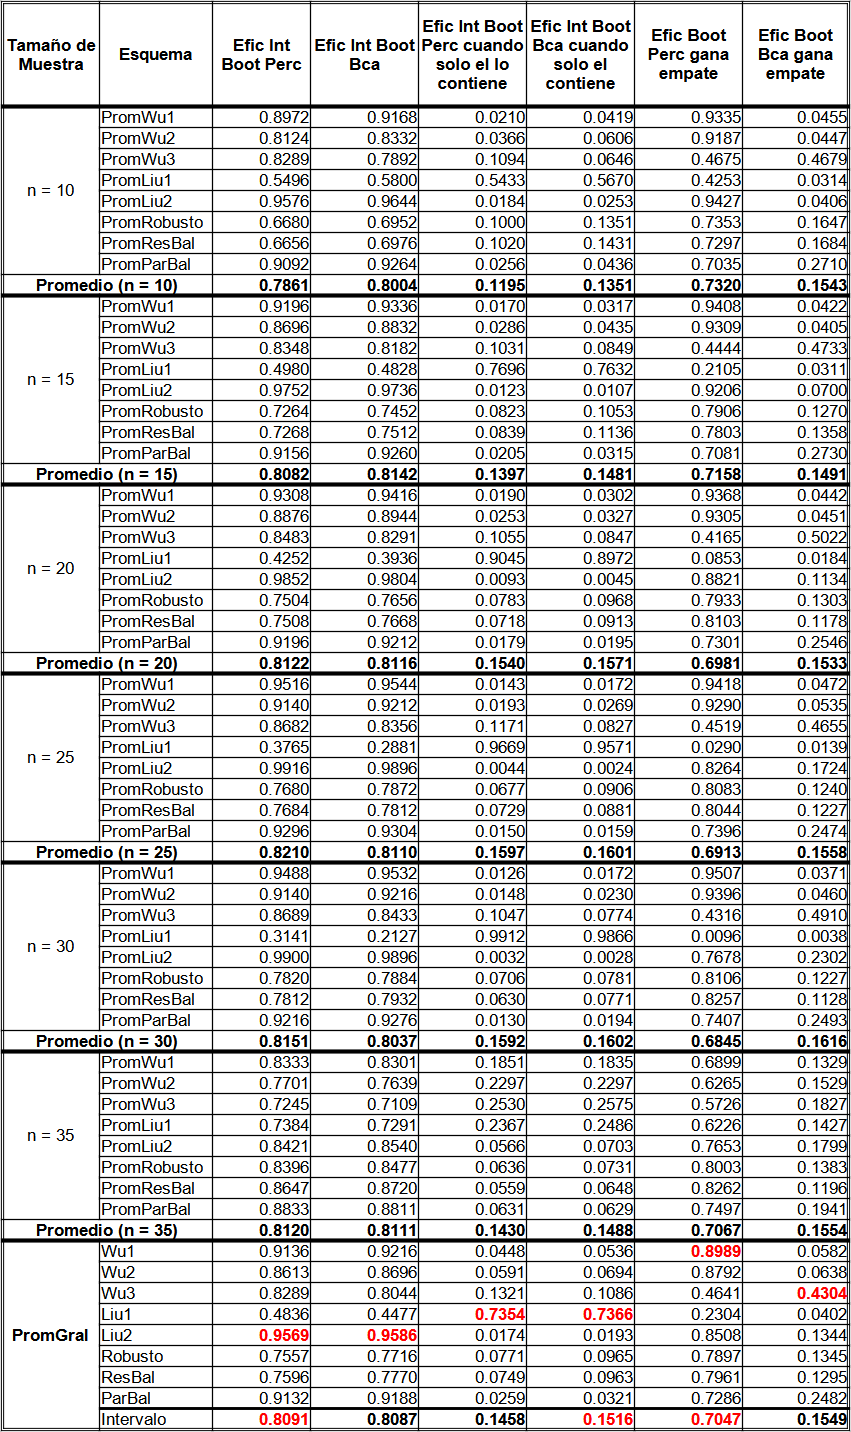
\includegraphics[width=0.75\linewidth]{img/EP_NVC_Efic_Boots.png} 
	\caption{Eficiencia promedio de los intervalos Bootstrap por tamaño de muestra y esquema de remuestreos para el caso EP-NVC.} 
	\label{fig:EP_NVC_Boots}
\end{figure}

\subsection{Eficiencia de los esquemas para el caso EP-NVC}

\begin{figure}[ht] 
	\centering 
	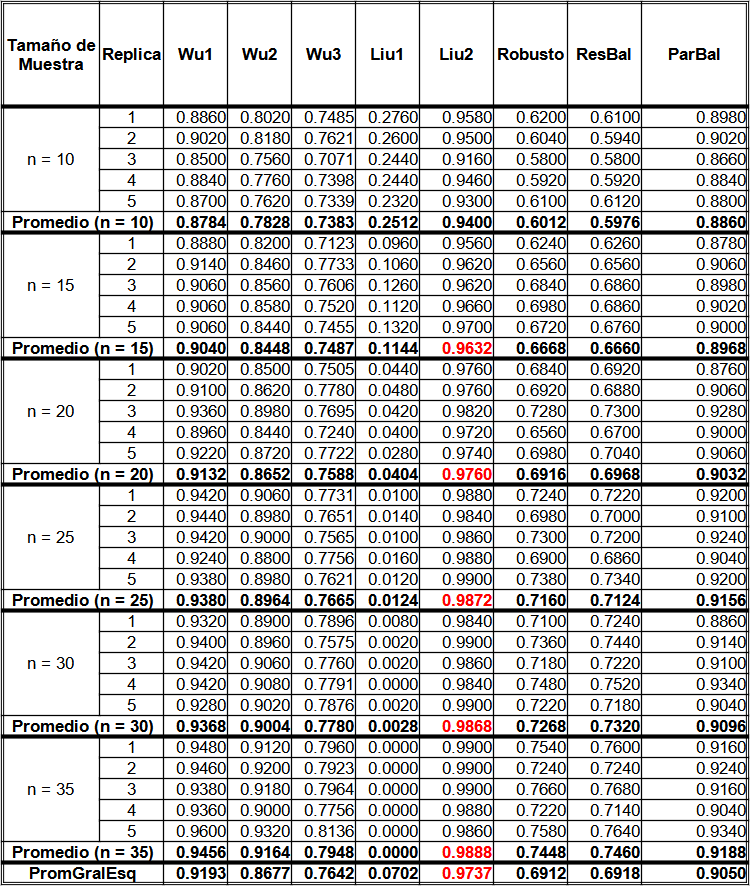
\includegraphics[width=0.9\linewidth]{img/EP_NVC_Efic_Esq.png} 
	\caption{Eficiencia promedio de los esquemas por tamaño de muestra y esquema de remuestreos para el caso EP-NVC.} 
	\label{fig:EP_NVC_Esq}
\end{figure}

EP-NNVC
\subsection{Eficiencia de los intervalos Bootstrap para el caso EP-NNVC}

\begin{figure}[ht] 
	\centering 
	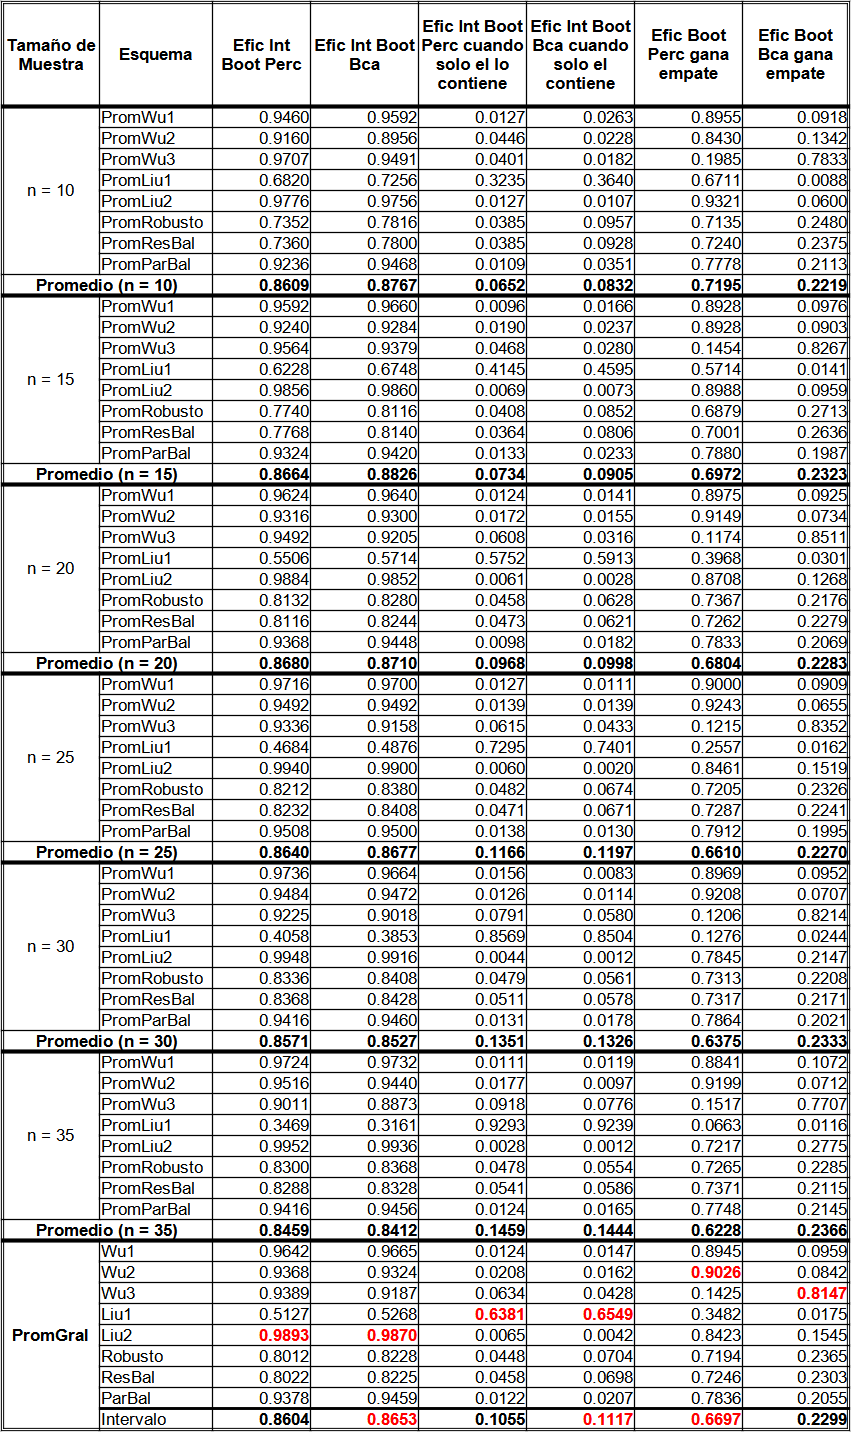
\includegraphics[width=0.75\linewidth]{img/EP_NNVC_Efic_Boots.png} 
	\caption{Eficiencia promedio de los intervalos Bootstrap por tamaño de muestra y esquema de remuestreos para el caso EP-NNVC.} 
	\label{fig:EP_NNVC_Boots}
\end{figure}

\subsection{Eficiencia de los esquemas para el caso EP-NNVC}

\begin{figure}[ht] 
	\centering 
	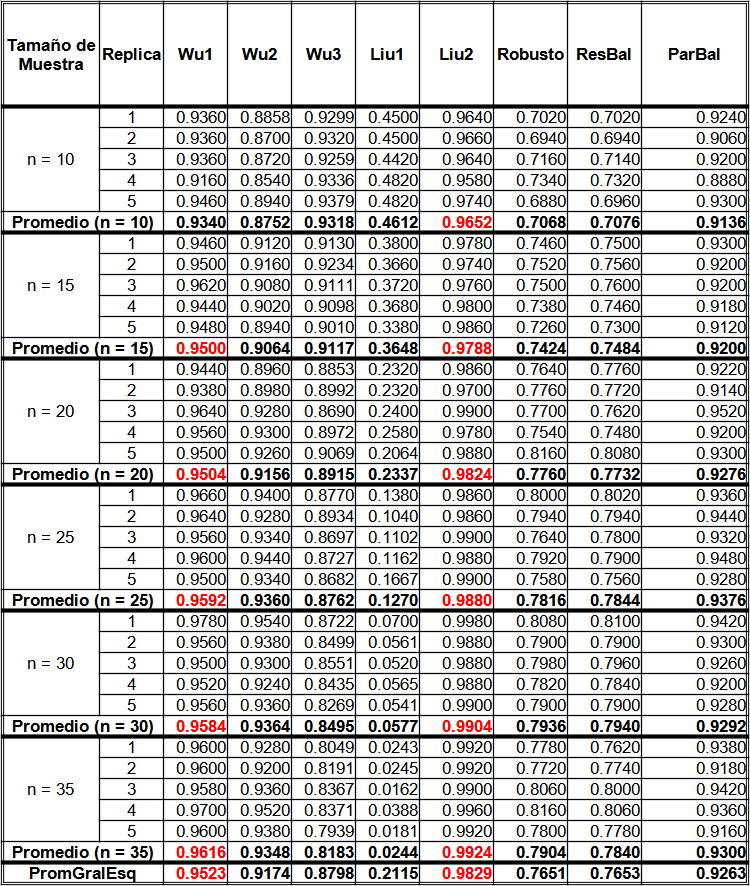
\includegraphics[width=0.9\linewidth]{img/EP_NNVC_Efic_Esq.png} 
	\caption{Eficiencia promedio de los esquemas por tamaño de muestra y esquema de remuestreos para el caso EP-NNVC.} 
	\label{fig:EP_NNVC_Esq}
\end{figure}

EP-NVD
\subsection{Eficiencia de los intervalos Bootstrap para el caso EP-NVD}

\begin{figure}[ht] 
	\centering 
	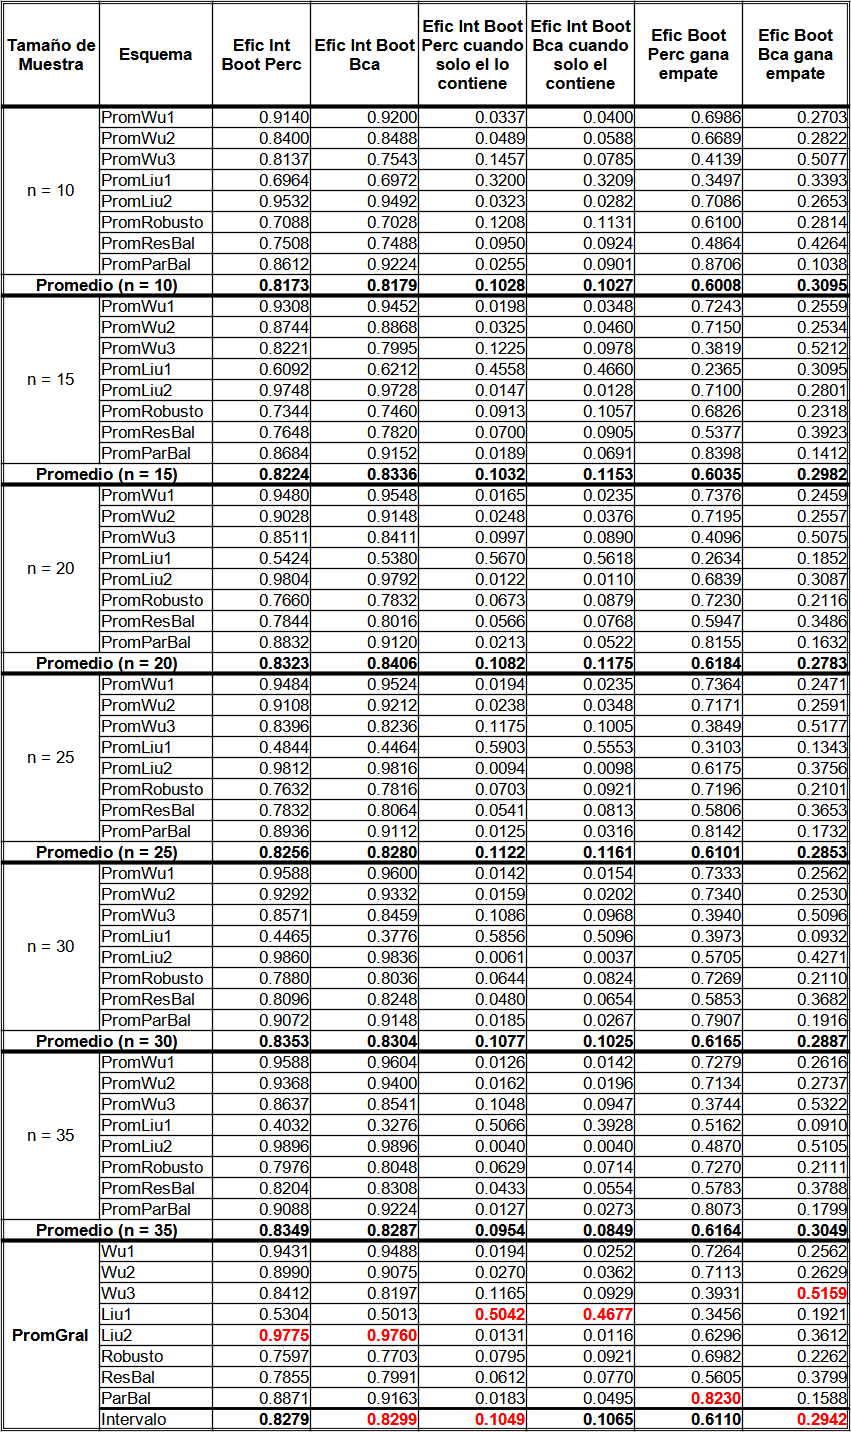
\includegraphics[width=0.75\linewidth]{img/EP_NVD_Efic_Boots.png} 
	\caption{Eficiencia promedio de los intervalos Bootstrap por tamaño de muestra y esquema de remuestreos para el caso EP-NVD.} 
	\label{fig:EP_NVD_Boots}
\end{figure}

\subsection{Eficiencia de los esquemas para el caso EP-NVD}

\begin{figure}[ht] 
	\centering 
	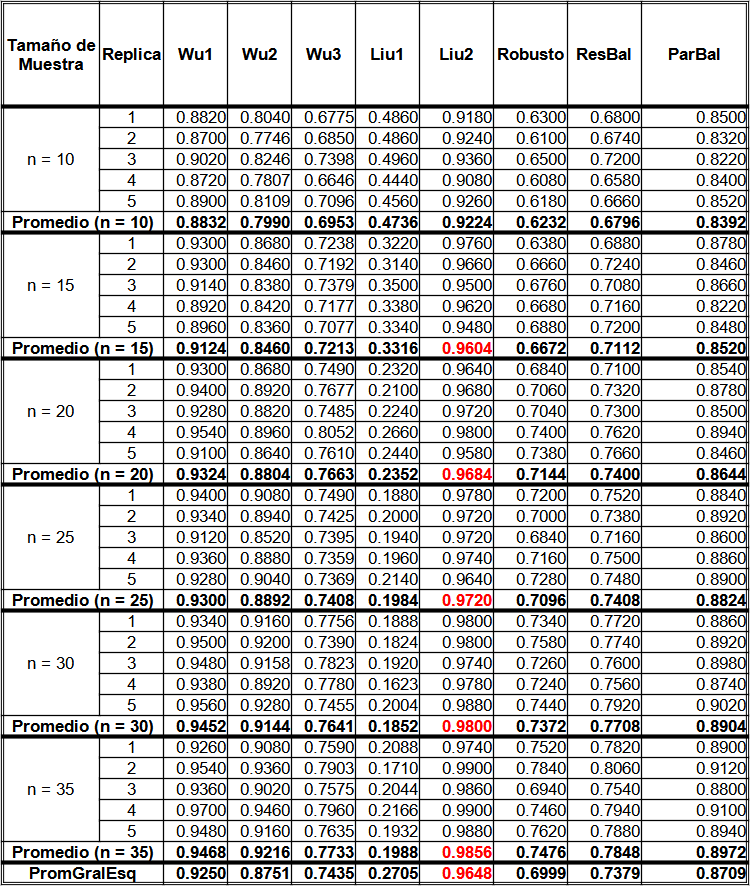
\includegraphics[width=0.9\linewidth]{img/EP_NVD_Efic_Esq.png} 
	\caption{Eficiencia promedio de los esquemas por tamaño de muestra y esquema de remuestreos para el caso EP-NVD.} 
	\label{fig:EP_NVD_Esq}
\end{figure}

EP-NNVD
\subsection{Eficiencia de los intervalos Bootstrap para el caso EP-NNVD}

\begin{figure}[ht] 
	\centering 
	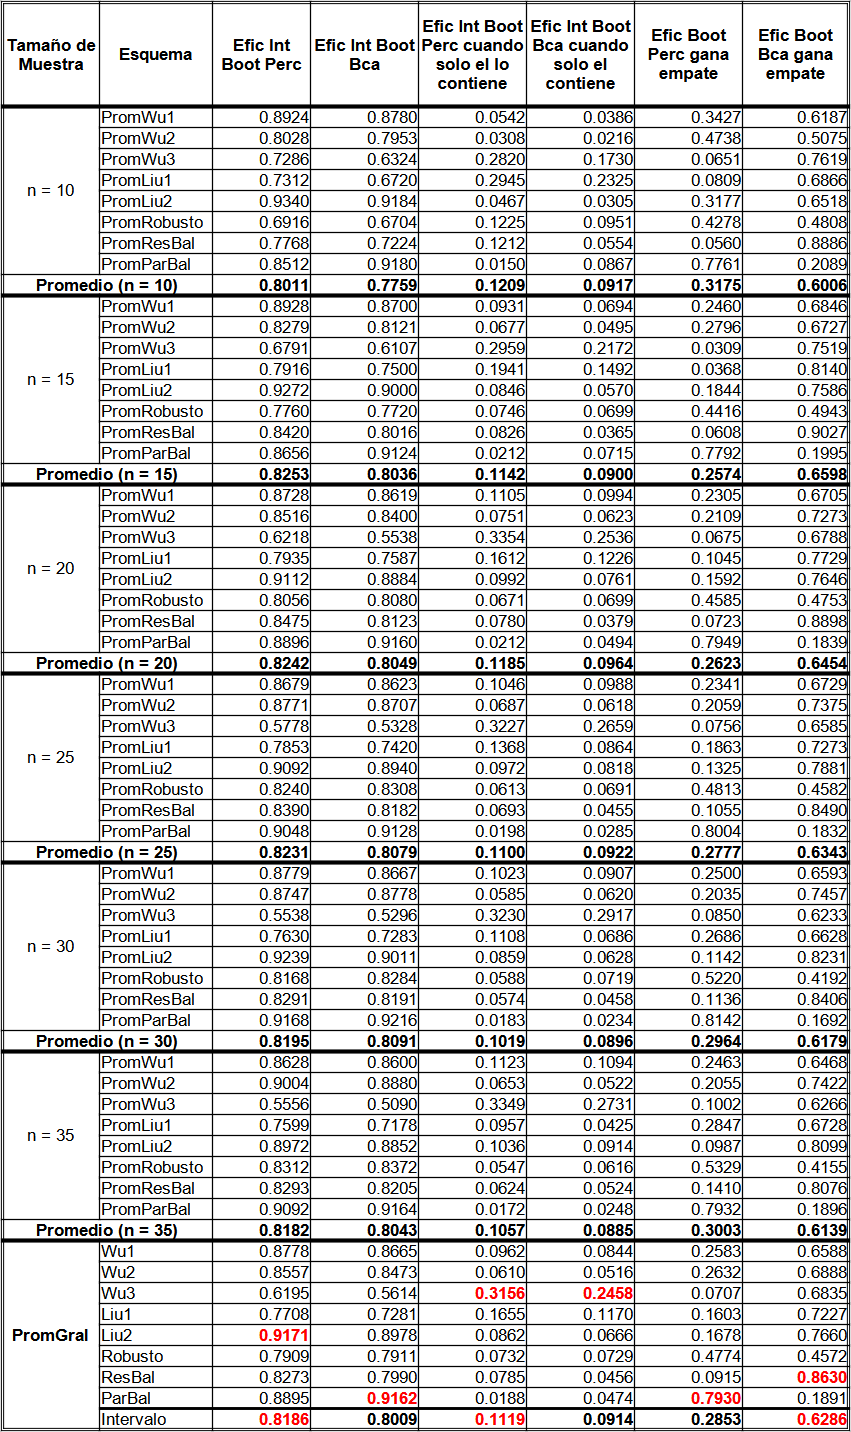
\includegraphics[width=0.75\linewidth]{img/EP_NNVD_Efic_Boots.png} 
	\caption{Eficiencia promedio de los intervalos Bootstrap por tamaño de muestra y esquema de remuestreos para el caso EP-NNVD.} 
	\label{fig:EP_NNVD_Boots}
\end{figure}

\subsection{Eficiencia de los esquemas para el caso EP-NNVD}

\begin{figure}[ht] 
	\centering 
	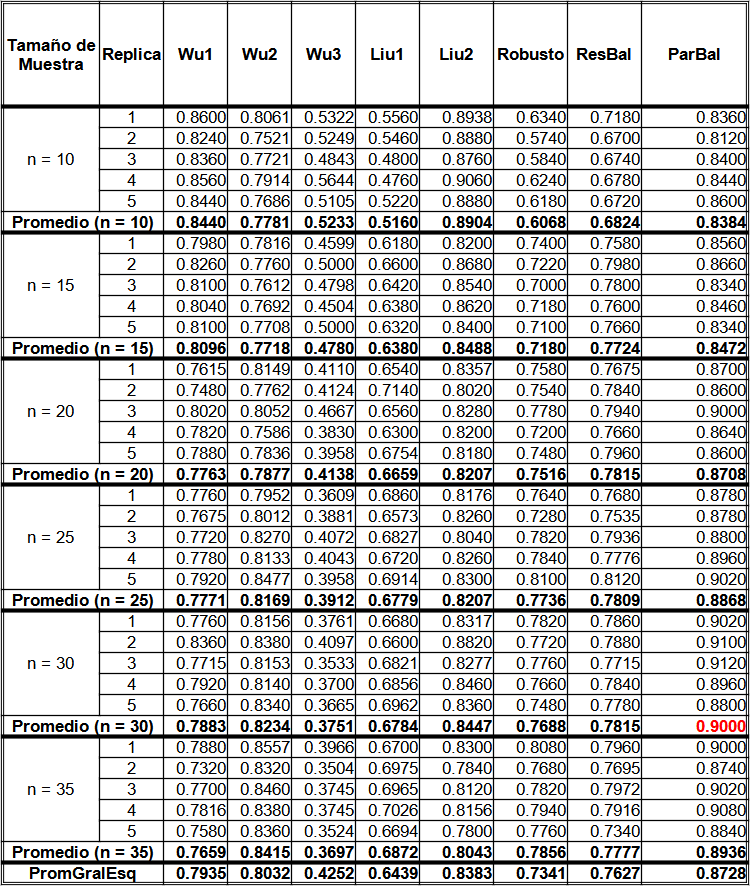
\includegraphics[width=0.9\linewidth]{img/EP_NNVD_Efic_Esq.png} 
	\caption{Eficiencia promedio de los esquemas por tamaño de muestra y esquema de remuestreos para el caso EP-NNVD.} 
	\label{fig:EP_NNVD_Esq}
\end{figure}

EP-Supuestos
\subsection{Promedio de supuestos para el caso EP}

\begin{figure}[ht] 
	\centering 
	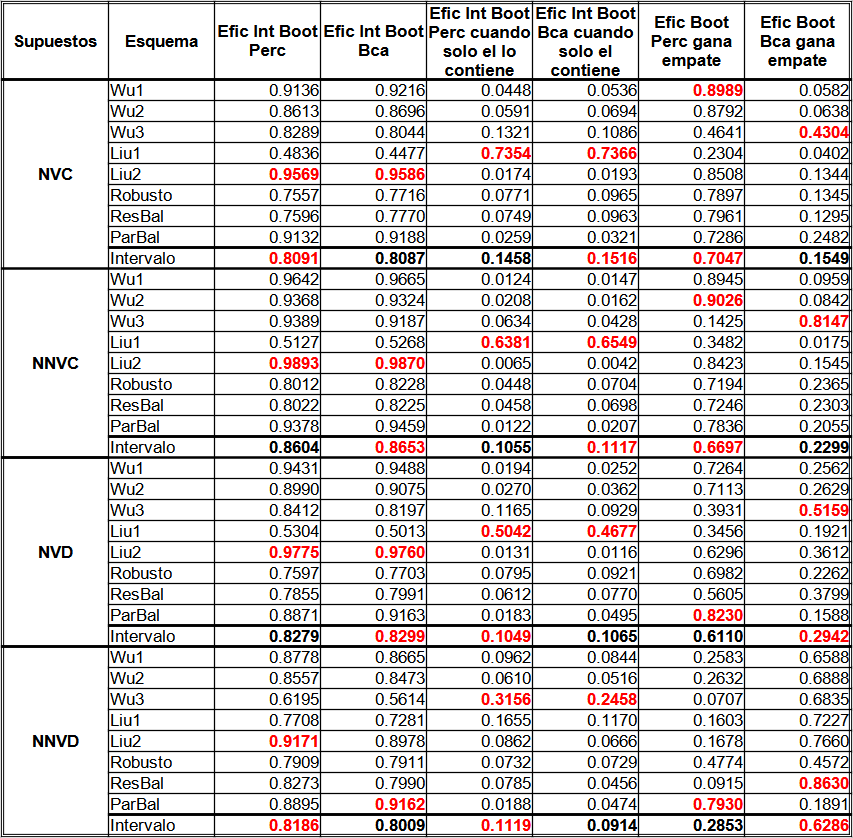
\includegraphics[width=0.9\linewidth]{img/EP_Prom_Supuestos.png} 
	\caption{Promedio de supuestos utilizados para el caso EP.} 
	\label{fig:EP_Supuestos}
\end{figure}

EI-NVC
\subsection{Eficiencia de los intervalos Bootstrap para el caso EI-NVC}

\begin{figure}[ht] 
	\centering 
	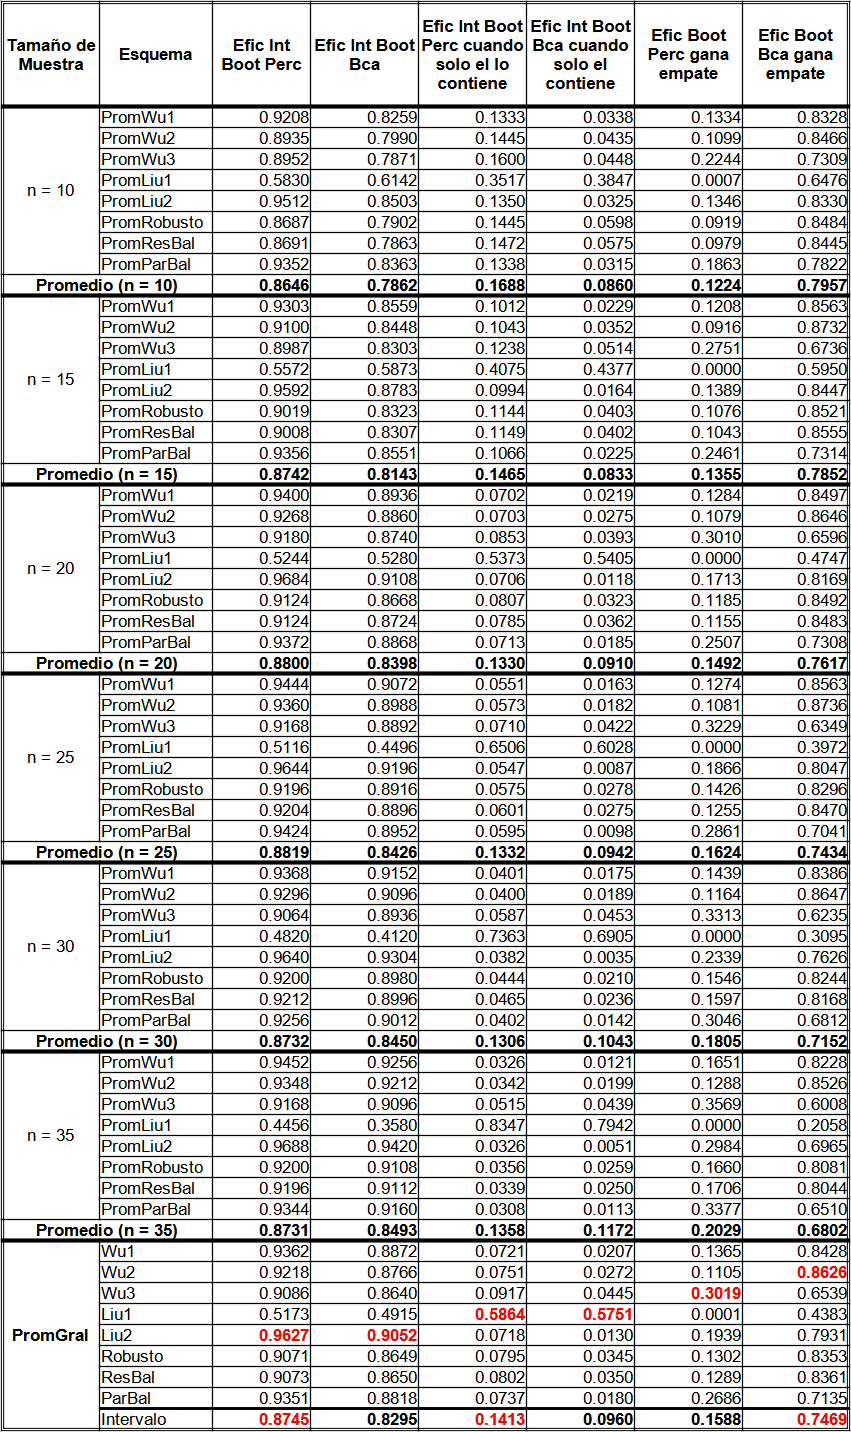
\includegraphics[width=0.75\linewidth]{img/EI_NVC_Efic_Boots.png} 
	\caption{Eficiencia promedio de los intervalos Bootstrap por tamaño de muestra y esquema de remuestreos para el caso EI-NVC.} 
	\label{fig:EI_NVC_Boots}
\end{figure}

\subsection{Eficiencia de los esquemas para el caso EI-NVC}

\begin{figure}[ht] 
	\centering 
	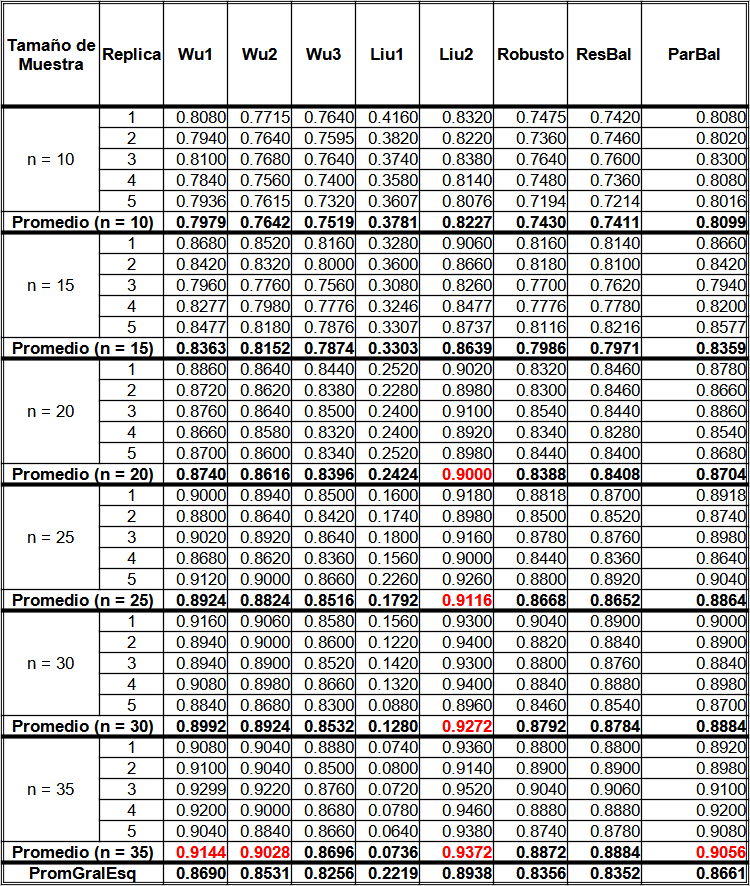
\includegraphics[width=0.9\linewidth]{img/EI_NVC_Efic_Esq.png} 
	\caption{Eficiencia promedio de los esquemas por tamaño de muestra y esquema de remuestreos para el caso EI-NVC.} 
	\label{fig:EI_NVC_Esq}
\end{figure}

EI-NNVC
\subsection{Eficiencia de los intervalos Bootstrap para el caso EI-NNVC}

\begin{figure}[ht] 
	\centering 
	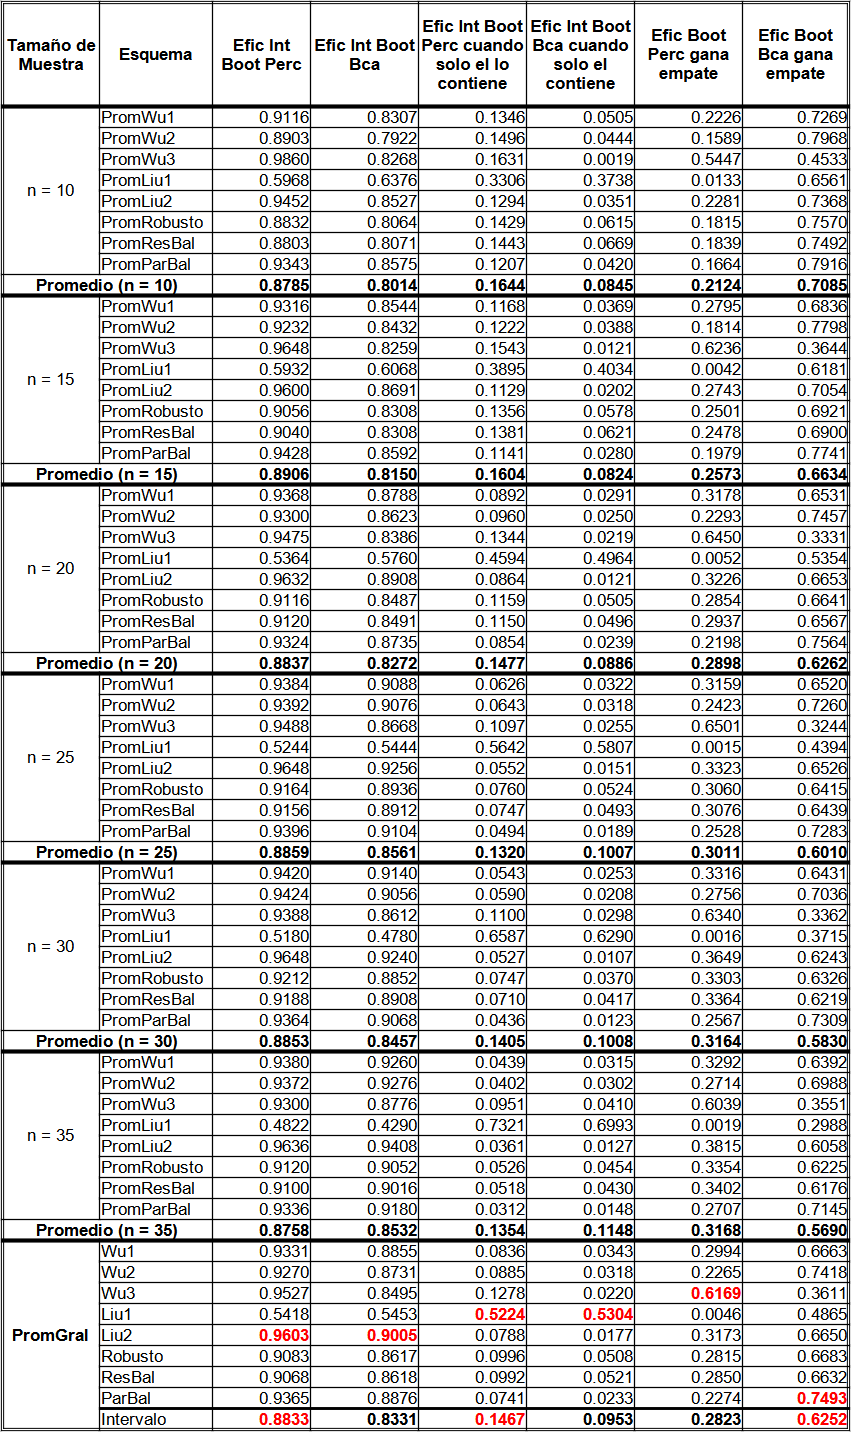
\includegraphics[width=0.75\linewidth]{img/EI_NNVC_Efic_Boots.png} 
	\caption{Eficiencia promedio de los intervalos Bootstrap por tamaño de muestra y esquema de remuestreos para el caso EI-NNVC.} 
	\label{fig:EI_NNVC_Boots}
\end{figure}

\subsection{Eficiencia de los esquemas para el caso EI-NNVC}

\begin{figure}[ht] 
	\centering 
	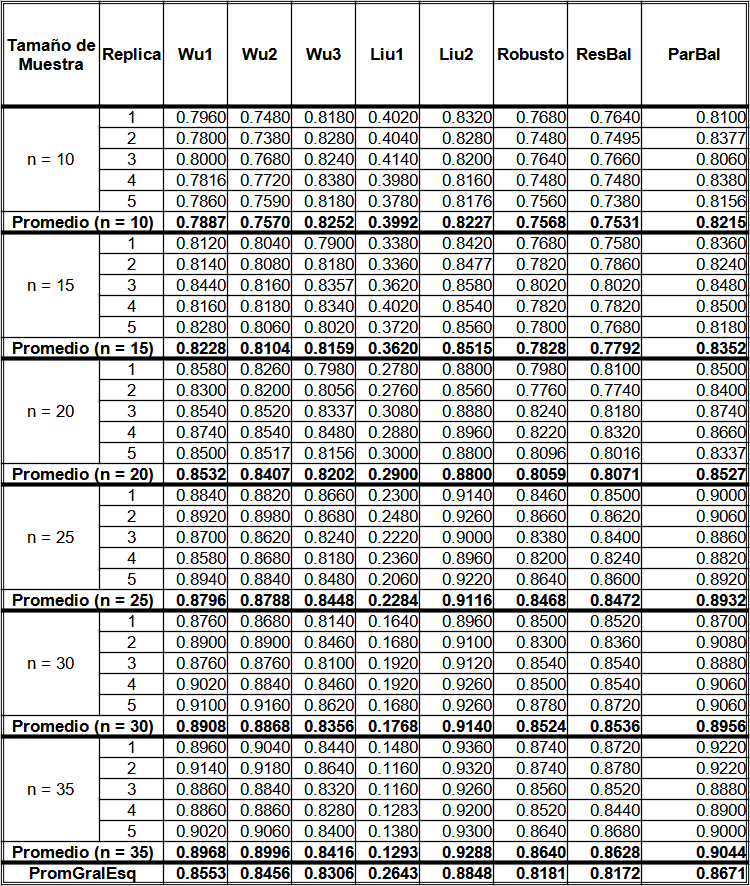
\includegraphics[width=0.9\linewidth]{img/EI_NNVC_Efic_Esq.png} 
	\caption{Eficiencia promedio de los esquemas por tamaño de muestra y esquema de remuestreos para el caso EI-NNVC.} 
	\label{fig:EI_NNVC_Esq}
\end{figure}

EI-NVD
\subsection{Eficiencia de los intervalos Bootstrap para el caso EI-NVD}

\begin{figure}[ht] 
	\centering 
	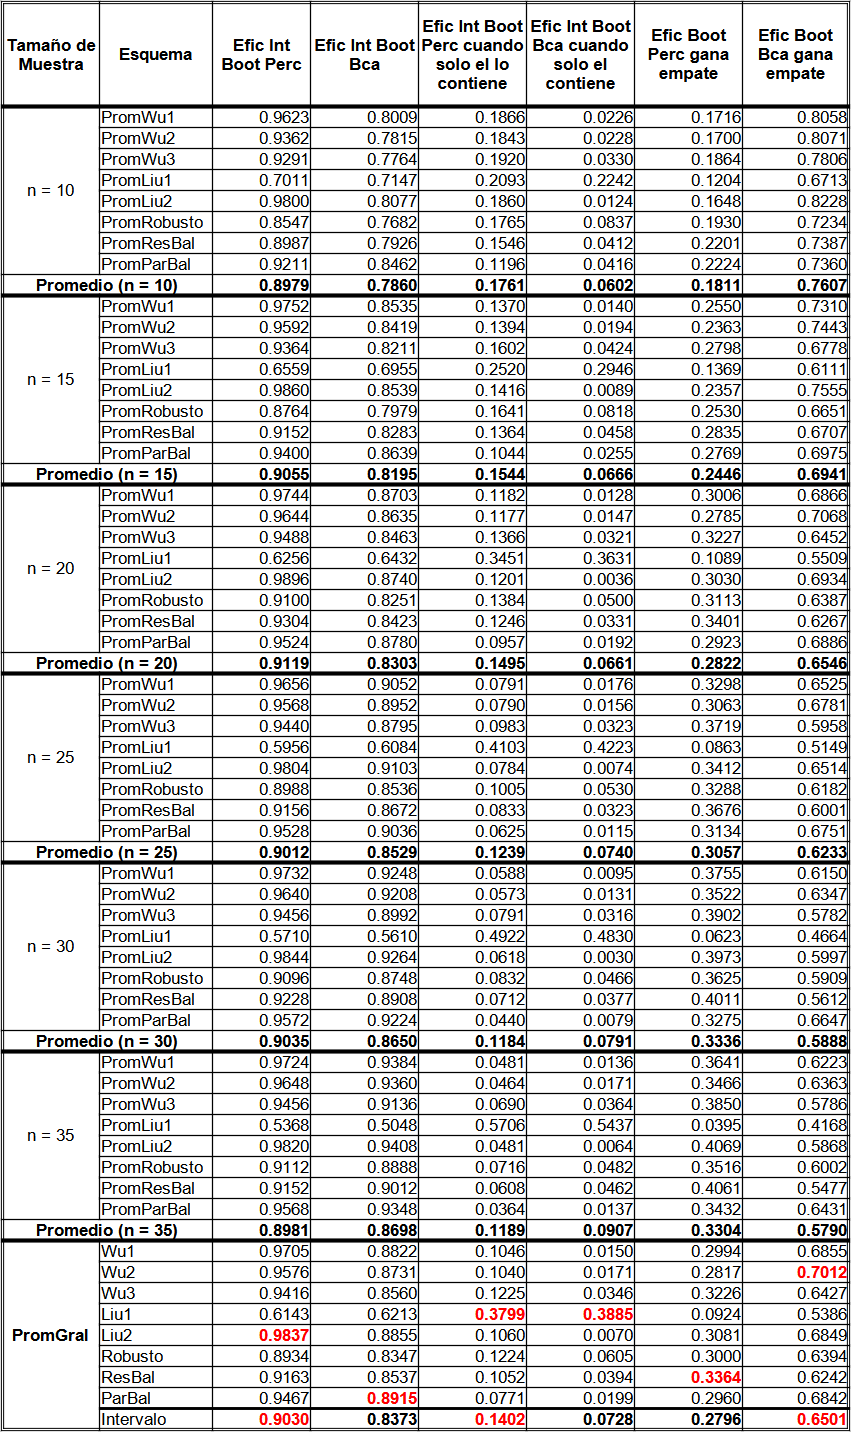
\includegraphics[width=0.75\linewidth]{img/EI_NVD_Efic_Boots.png} 
	\caption{Eficiencia promedio de los intervalos Bootstrap por tamaño de muestra y esquema de remuestreos para el caso EI-NVD.} 
	\label{fig:EI_NVD_Boots}
\end{figure}

\subsection{Eficiencia de los esquemas para el caso EI-NVD}

\begin{figure}[ht] 
	\centering 
	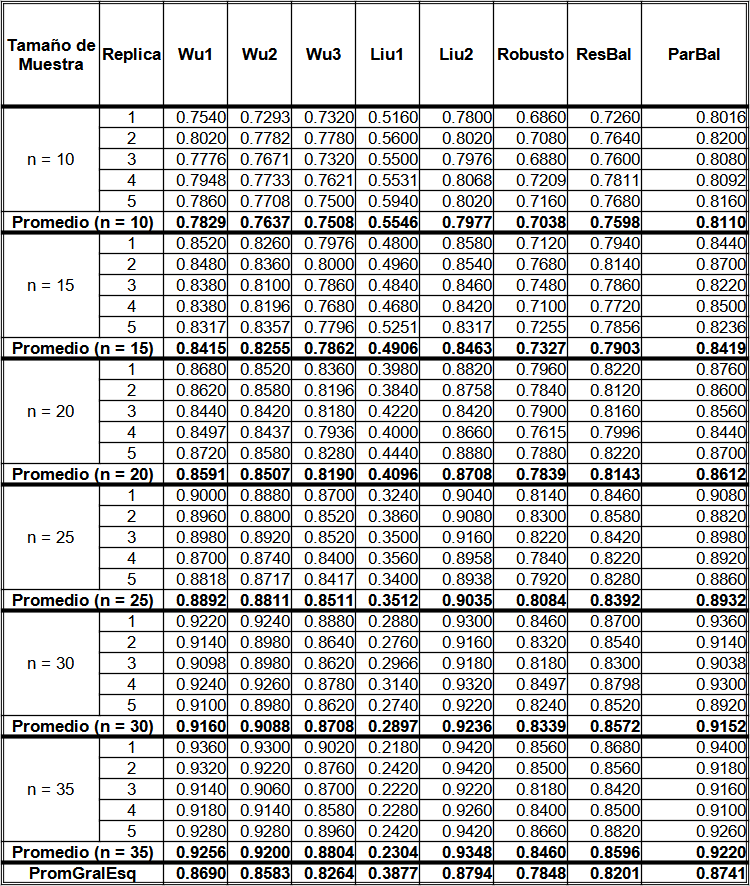
\includegraphics[width=0.9\linewidth]{img/EI_NVD_Efic_Esq.png} 
	\caption{Eficiencia promedio de los esquemas por tamaño de muestra y esquema de remuestreos para el caso EI-NVD.} 
	\label{fig:EI_NVD_Esq}
\end{figure}

EI-NNVD
\subsection{Eficiencia de los intervalos Bootstrap para el caso EI-NNVD}

\begin{figure}[ht] 
	\centering 
	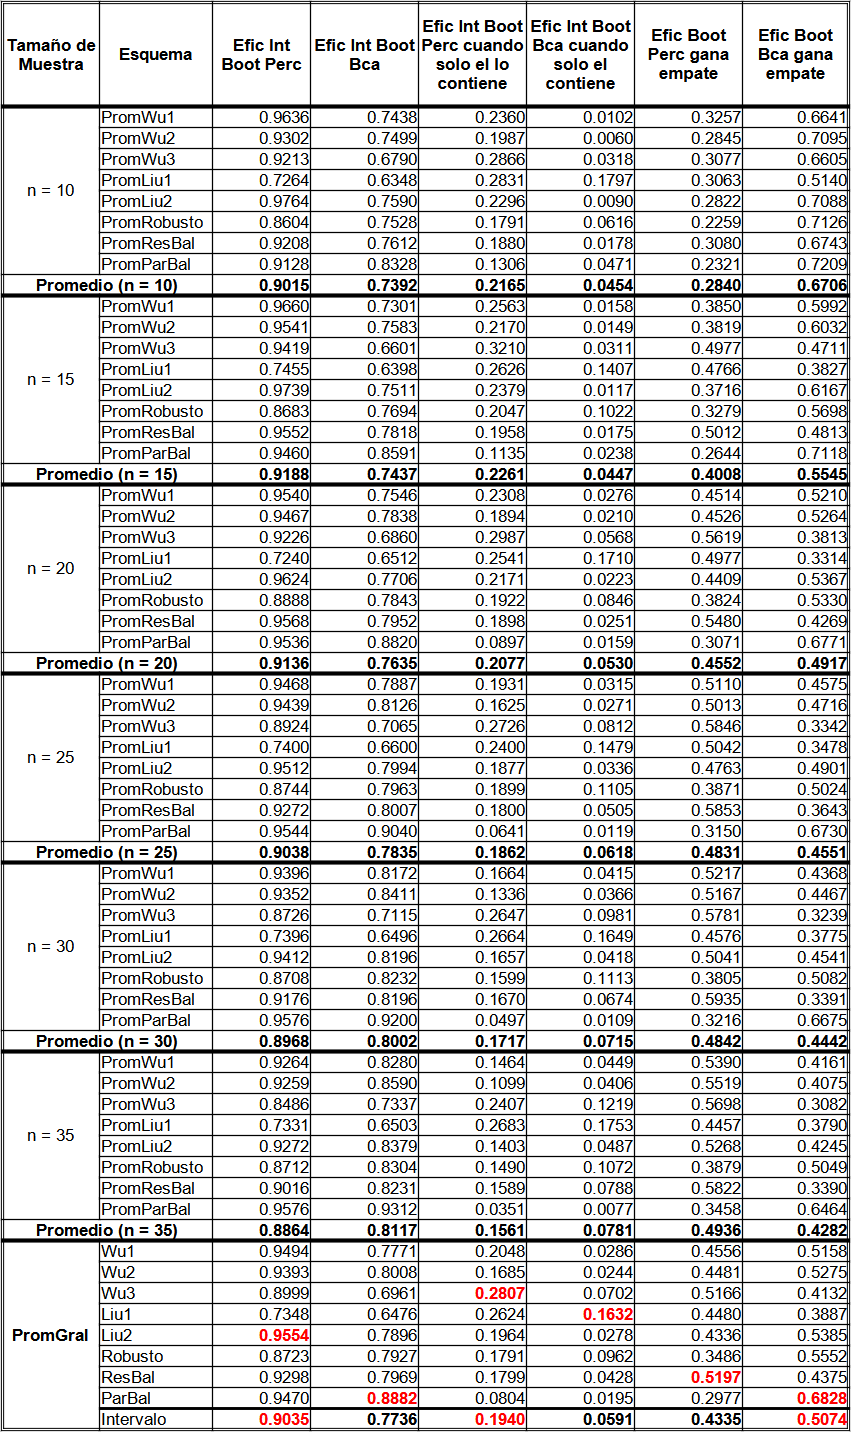
\includegraphics[width=0.75\linewidth]{img/EI_NNVD_Efic_Boots.png} 
	\caption{Eficiencia promedio de los intervalos Bootstrap por tamaño de muestra y esquema de remuestreos para el caso EI-NNVD.} 
	\label{fig:EI_NNVD_Boots}
\end{figure}

\subsection{Eficiencia de los esquemas para el caso EI-NNVD}

\begin{figure}[ht] 
	\centering 
	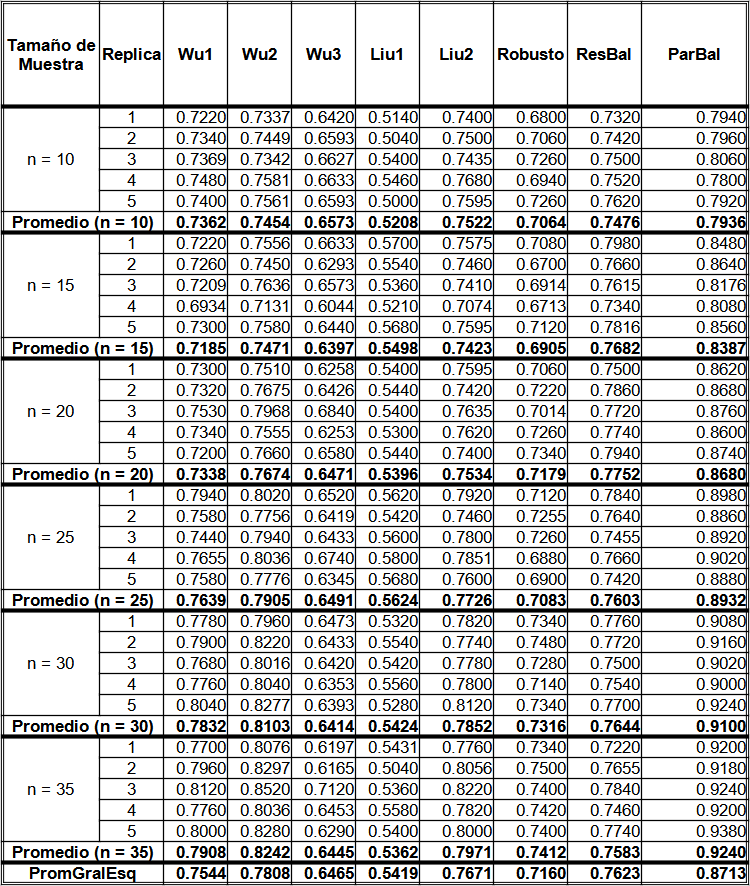
\includegraphics[width=0.9\linewidth]{img/EI_NNVD_Efic_Esq.png} 
	\caption{Eficiencia promedio de los esquemas por tamaño de muestra y esquema de remuestreos para el caso EI-NNVD.} 
	\label{fig:EI_NNVD_Esq}
\end{figure}

EI-Supuestos
\subsection{Promedio de supuestos para el caso EI}

\begin{figure}[ht] 
	\centering 
	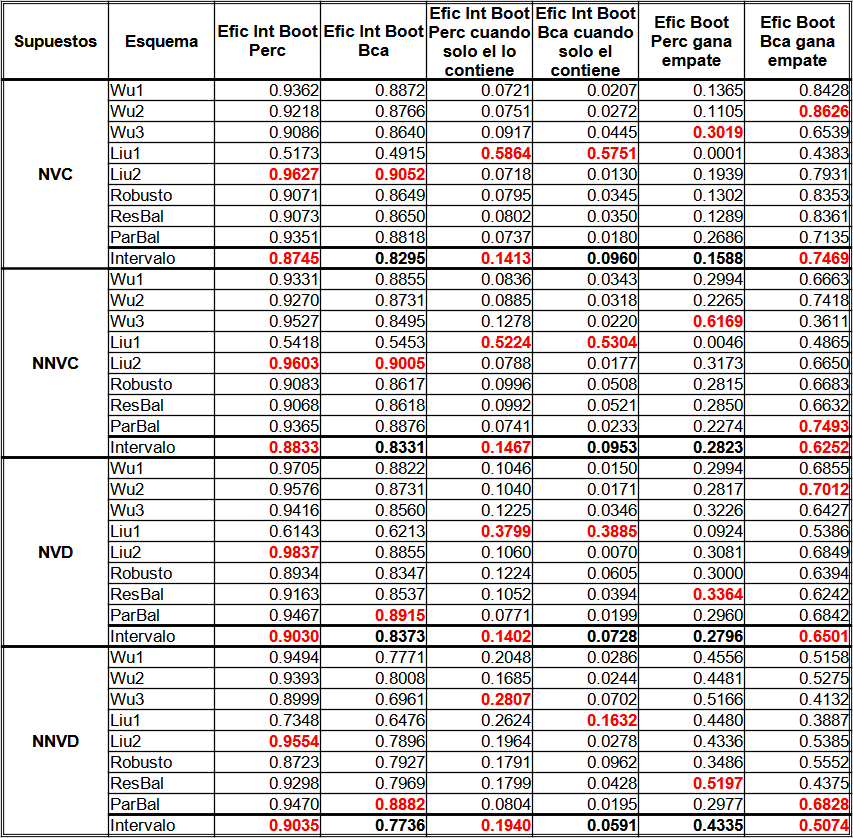
\includegraphics[width=0.8\linewidth]{img/EI_Prom_Supuestos.png} 
	\caption{Promedio de supuestos utilizados para el caso EI.} 
	\label{fig:EI_Supuestos}
\end{figure}

